\documentclass[aspectratio=169,11pt]{beamer}

% Shared style (ib-tutorials.sty at the repo root).
\makeatletter\def\input@path{{./}{../}}\makeatother
\usepackage{ib-tutorials}

\usepackage[utf8]{inputenc}
\usepackage{amsmath,amssymb}
\usepackage{booktabs}
\usepackage{array}
\usepackage{graphicx}
\usepackage{xcolor}
\usepackage{listings}
\usepackage{tikz}
\usetikzlibrary{arrows.meta,positioning,shapes.geometric,fit,calc}
\usepackage{hyperref}

\newcommand{\sourcecredit}[1]{\vfill\hfill{\tiny\textcolor{DarkGray}{#1}}}
\newcolumntype{L}[1]{>{\raggedright\arraybackslash}p{#1}}

\lstset{
  basicstyle=\ttfamily\scriptsize\color{BlackGray},
  keywordstyle=\color{NavyBlue}\bfseries,
  commentstyle=\color{DarkGray}\itshape,
  stringstyle=\color{OliveGreen},
  showstringspaces=false,
  columns=fullflexible,
  keepspaces=true,
  frame=single,
  framerule=0.4pt,
  rulecolor=\color{LightGray},
  backgroundcolor=\color{LightGray!30},
  xleftmargin=0.25em,
  xrightmargin=0.25em,
  breaklines=true,
  breakatwhitespace=true
}
\lstdefinestyle{shell}{morecomment=[l]{\#}}
\lstdefinestyle{cpp}{language=C++,morekeywords={nullptr}}
\lstdefinestyle{tiny}{basicstyle=\ttfamily\tiny\color{BlackGray}}
\lstdefinestyle{slurm}{}

\title[Building and running]{Building and running an IBAMR application}
\subtitle{From source files to results, on a laptop or on Puma}
\author[Miller]{Laura A. Miller}
\institute[UArizona]{Department of Mathematics, University of Arizona}
\date{Using IB Software \textbullet\ Part I \textbullet\ Chapter 3}

\tikzset{
  file/.style={draw=DarkGray,rounded corners=1pt,fill=LightGray!45,align=center,inner sep=3pt,font=\scriptsize},
  action/.style={draw=RubineRed,thick,rounded corners=1pt,fill=RubineRed!8,align=center,inner sep=3pt,font=\scriptsize},
  arr/.style={-{Stealth[length=2mm]},DarkGray}
}

\begin{document}

% 1
\begin{frame}[plain]
\maketutorialtitlepanel{%
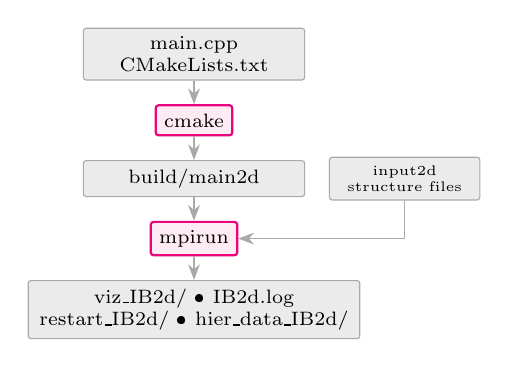
\begin{tikzpicture}[node distance=3mm]
  \node[file,text width=26mm] (src) {\code{main.cpp}\\\code{CMakeLists.txt}};
  \node[action,below=of src] (cm) {\code{cmake}};
  \node[file,below=of cm,text width=26mm] (exe) {\code{build/main2d}};
  \node[file,right=3mm of exe,text width=17mm,font=\tiny] (inp) {\code{input2d}\\structure files};
  \node[action,below=of exe] (mpi) {\code{mpirun}};
  \node[file,below=of mpi,text width=40mm] (out) {\code{viz\_IB2d/} \textbullet\ \code{IB2d.log}\\\code{restart\_IB2d/} \textbullet\ \code{hier\_data\_IB2d/}};
  \draw[arr] (src)--(cm); \draw[arr] (cm)--(exe); \draw[arr] (exe)--(mpi);
  \draw[arr] (inp) |- (mpi); \draw[arr] (mpi)--(out);
\end{tikzpicture}}
\end{frame}

% 2
\begin{frame}{Learning goals}
By the end of this chapter you should be able to:
\begin{enumerate}
  \item build an IBAMR program with CMake, in 2D or 3D;
  \item run it with MPI and read what it prints and logs;
  \item find your way around an input file and change it safely;
  \item run on Puma with a batch script, follow the job, and restart it;
  \item estimate how long a run will take and how much disk it needs;
  \item port an older course example to current IBAMR;
  \item run a parameter sweep as a Slurm job array.
\end{enumerate}
\vspace{3mm}
\begin{punchbox}
\small The examples are the three starter examples of this tutorial: the rubber band (IB/01), the pulsatile channel (IB/02) and the tethered plate (IBFE/01). Every command and message on these slides was run and recorded with IBAMR 0.16.0 and 0.19.0.
\end{punchbox}
\end{frame}

% 3
\begin{frame}[fragile]{What an IBAMR application is}
\begin{columns}[T,onlytextwidth]
\begin{column}{0.49\textwidth}
\begin{lstlisting}
examples/IB/01-rubber-band/
  CMakeLists.txt          how to build
  main.cpp                the program
  input2d                 all the settings
  rubber_band_512.vertex  the structure:
  rubber_band_512.spring    points and springs
  generate_mesh2d.m       makes those files
  job.slurm               batch script for Puma
  README.md
\end{lstlisting}
\end{column}
\begin{column}{0.48\textwidth}
\begin{itemize}\small
  \item IBAMR is a \al{library}. Your application is a short C++ program, \code{main.cpp}, that sets up IBAMR's objects and runs the time-step loop.
  \item Almost every choice lives in the \al{input file}: physical constants, grid, solver settings, output.
  \item The structure comes from files (\code{.vertex}, \code{.spring}, \ldots) or, for IBFE, a finite element mesh.
  \item Most course examples share one program and differ in their input and structure files. IB/01 and IB/02 use the same \code{main.cpp}.
\end{itemize}
\end{column}
\end{columns}
\end{frame}

% 4
\begin{frame}[fragile]{The old way to build: a Makefile}
Until 2025 every course example came with a \code{Makefile} that pointed at one particular IBAMR install. The 2024 course instructions said to edit these lines:
\begin{lstlisting}[style=shell]
IBAMR_SRC_DIR = /groups/lauram9/ib10/ibamr/IBAMR
IBAMR_BUILD_DIR = /groups/lauram9/ib10/ibamr/ibamr-objs-opt
LIBSNEW = $(LIBS) -lnetcdf -lcurl
...
include $(IBAMR_BUILD_DIR)/config/make.inc
\end{lstlisting}
With an autoibamr install, \code{make main2d} stops at once:
\begin{lstlisting}
Makefile:27: /contrib/lauram9/ibamr/IBAMR-0.7.1/config/make.inc: No such file or directory
make: *** No rule to make target '/contrib/lauram9/ibamr/IBAMR-0.7.1/config/make.inc'.  Stop.
\end{lstlisting}
\begin{itemize}\small
  \item autoibamr builds IBAMR with CMake, which creates no \code{make.inc}.
  \item The next release, IBAMR 0.20 (in development in 2026), removes Makefile builds of IBAMR altogether.
  \item So every example in this tutorial now builds with CMake. The Makefiles are kept in \code{examples/legacy/} and in Part X.
\end{itemize}
\end{frame}

% 5
\begin{frame}[fragile]{The new way: \code{CMakeLists.txt}, line by line}
\begin{lstlisting}[style=shell]
cmake_minimum_required(VERSION 3.15...3.30)
project(ib01_rubber_band LANGUAGES C CXX)

find_package(IBAMR 0.16.0 REQUIRED)

add_executable(main2d main.cpp)
target_link_libraries(main2d PRIVATE IBAMR::IBAMR2d)
\end{lstlisting}
\small
\begin{tabular}{@{}L{0.33\textwidth}L{0.63\textwidth}@{}}
\toprule
Line & What it does \\
\midrule
\code{cmake\_minimum\_required} & the range turns on newer CMake rules, which also silences two harmless warnings from IBAMR's CMake files \\
\code{project} & names the project; C and C++ compilers are needed \\
\code{find\_package(IBAMR 0.16.0 \ldots)} & finds IBAMR 0.16.0 or newer, through \code{IBAMR\_ROOT} from \code{enable.sh} \\
\code{add\_executable} & the program to build and its source files \\
\code{target\_link\_libraries} & links IBAMR and everything it needs; \code{IBAMR2d} also sets the dimension, \code{NDIM = 2} \\
\bottomrule
\end{tabular}
\end{frame}

% 6
\begin{frame}[fragile]{Configure, then build}
From the example's folder, after loading the install (chapter 2):
\begin{lstlisting}[style=shell]
source ~/autoibamr/configuration/enable.sh     # on Puma: module load gnu13 openmpi5 first
cmake -S . -B build -DCMAKE_BUILD_TYPE=Release # configure: once per build folder
cmake --build build -j 4                       # compile: after every change to main.cpp
\end{lstlisting}
The last lines you should see (from the rubber band with IBAMR 0.19.0):
\begin{lstlisting}[style=tiny]
-- Configuring done (5.6s)
-- Generating done (0.0s)
-- Build files have been written to: /root/work/0.19.0/ib01/build
[ 50%] Building CXX object CMakeFiles/main2d.dir/main.cpp.o
[100%] Linking CXX executable main2d
[100%] Built target main2d
\end{lstlisting}
\begin{itemize}\small
  \item \code{-S .} is the source folder and \code{-B build} the build folder. The program ends up as \code{build/main2d}.
  \item Changing \code{input2d} needs no rebuild; changing \code{main.cpp} does.
  \item Start over by deleting the \code{build} folder.
\end{itemize}
\end{frame}

% 7
\begin{frame}[fragile]{3D programs, extra source files, debugging}
\begin{columns}[T,onlytextwidth]
\begin{column}{0.49\textwidth}
\begin{block}{A 3D program}
\begin{lstlisting}[style=shell]
add_executable(main3d main.cpp)
target_link_libraries(main3d PRIVATE
                      IBAMR::IBAMR3d)
\end{lstlisting}
\small The same \code{main.cpp} can build both: \code{NDIM} is 2 or 3 depending on the library it links.
\end{block}
\begin{block}{Extra source files}
\begin{lstlisting}[style=shell]
add_executable(main2d main.cpp
    update_target_point_positions.cpp)
\end{lstlisting}
\small List every \code{.cpp} file your program needs (IB/03 and IB/04 move target points this way).
\end{block}
\end{column}
\begin{column}{0.47\textwidth}
\begin{block}{Debugging your own code}
\small Configure a second build folder:
\begin{lstlisting}[style=shell]
cmake -S . -B build-debug \
      -DCMAKE_BUILD_TYPE=Debug
\end{lstlisting}
\small This adds debug symbols and turns off optimization for \emph{your} code. To also check IBAMR's internal assertions, build against a debug install of IBAMR (chapter 2, \code{--enable-debugging}). Debug runs are much slower.
\end{block}
\end{column}
\end{columns}
\end{frame}

% 8
\begin{frame}[fragile]{Running a simulation}
\begin{lstlisting}[style=shell]
mpirun -np 4 ./build/main2d input2d                    # a new run on 4 processes
mpirun -np 4 ./build/main2d input2d restart_IB2d 1000  # continue from step 1000
\end{lstlisting}
\begin{itemize}
  \item \code{-np 4} starts 4 MPI processes. IBAMR divides the grid and the structure among them.
  \item Run from the example's folder: the input file names the structure files without a path, and output folders are made where you start.
  \item The second form restarts from a saved state, explained later in this chapter.
  \item On Puma, this line goes \emph{inside} a batch script or an interactive session, never on the login node.
\end{itemize}
\vspace{2mm}
\begin{punchbox}
\small The rubber band's full run, 20{,}000 time steps, took 166~s with IBAMR 0.16.0 and 181~s with 0.19.0 on 4 cores of a desktop PC (WSL).
\end{punchbox}
\end{frame}

% 9
\begin{frame}[fragile]{What the screen shows}
\begin{columns}[T,onlytextwidth]
\begin{column}{0.56\textwidth}
\begin{lstlisting}[style=tiny]
IBStandardInitializer:  Reading from input files.
  base filename: rubber_band_512
  assigned to level 3 of the Cartesian grid patch hierarchy

Writing visualization files...

+++++++++++++++++++++++++++++++++++++++++++++++++++
At beginning of timestep # 0
Simulation time is 0

At end       of timestep # 0
Simulation time is 0.0001
+++++++++++++++++++++++++++++++++++++++++++++++++++
\end{lstlisting}
\end{column}
\begin{column}{0.41\textwidth}
\begin{itemize}\small
  \item First IBAMR reads the structure files and places the structure on the finest grid level (here level 3).
  \item It writes the first VisIt frame, at time 0.
  \item Then it prints two lines at the start and end of every time step.
  \item The rubber band also prints \code{integral\{F\}}, the sum of its forces, every 400 steps; that line comes from the example's own \code{output\_data} function.
\end{itemize}
\end{column}
\end{columns}
\end{frame}

% 10
\begin{frame}[fragile]{What the log file shows: one IB time step}
\code{IB2d.log} (set by \code{log\_file\_name}) records each stage of every step. Step 100 of the rubber band:
\begin{lstlisting}[style=tiny]
IBHierarchyIntegrator::advanceHierarchy(): time interval = [0.01,0.0101], dt = 0.0001
IBHierarchyIntegrator::preprocessIntegrateHierarchy(): performing Lagrangian forward Euler step
IBHierarchyIntegrator::integrateHierarchy(): computing Lagrangian force
IBHierarchyIntegrator::integrateHierarchy(): spreading Lagrangian force to the Eulerian grid
IBHierarchyIntegrator::integrateHierarchy(): solving the incompressible Navier-Stokes equations
INSStaggeredHierarchyIntegrator::integrateHierarchy(): stokes solve number of iterations = 3
INSStaggeredHierarchyIntegrator::integrateHierarchy(): stokes solve residual norm        = 0.658181
IBHierarchyIntegrator::integrateHierarchy(): interpolating Eulerian velocity to the Lagrangian mesh
IBHierarchyIntegrator::integrateHierarchy(): performing Lagrangian midpoint-rule step
IBHierarchyIntegrator::postprocessIntegrateHierarchy(): CFL number = 0.00987275
IBHierarchyIntegrator::postprocessIntegrateHierarchy(): Eulerian estimate of upper bound on IB point displacement since last regrid = 0.450684
\end{lstlisting}
\begin{itemize}\small
  \item The stages are the IB method itself: compute the structure's forces, \al{spread} them to the grid, solve the fluid equations, \al{interpolate} the velocity back, and move the points.
  \item Watch the \textbf{CFL number} and the \textbf{number of Stokes iterations}. A CFL number that keeps growing or iteration counts that climb are early signs of trouble (chapter 16).
\end{itemize}
\end{frame}

% 11
\begin{frame}{Where the output goes}
\footnotesize
\begin{tabular}{@{}L{0.40\textwidth}L{0.56\textwidth}@{}}
\toprule
Path & What it holds \\
\midrule
\code{viz\_IB2d/dumps.visit} & list of fluid frames for VisIt: \code{U}, \code{P}, \code{Omega}, \ldots{} on the adaptive grid \\
\code{viz\_IB2d/lag\_data.visit} & list of structure frames for VisIt (Lagrangian points) \\
\code{viz\_IB2d/visit\_dump.NNNNN/} & one fluid frame per folder; \code{NNNNN} is the time step \\
\code{viz\_IB2d/lag\_data.cycle\_NNNNNN/} & one structure frame per folder \\
\code{viz\_IB2d/output.ex2} & IBFE only: the finite element mesh and its data, all frames in one file \\
\code{hier\_data\_IB2d/} & data written by the example's \code{output\_data} (rubber band: positions \code{X.NNNNN} and forces \code{F.NNNNN}) \\
\code{restart\_IB2d/restore.NNNNNN/} & saved states for restarting \\
\code{IB2d.log} & the log file \\
\bottomrule
\end{tabular}
\vspace{3mm}

Sizes from the full runs: rubber band 39~MB of VisIt files for 51 frames plus 1.4~MB of data files; tethered plate 14~MB for 41 frames.
\end{frame}

% 12
\begin{frame}[fragile]{The input file: variables and blocks}
\begin{columns}[T,onlytextwidth]
\begin{column}{0.50\textwidth}
\begin{lstlisting}
// physical parameters
L = 1.0                // domain length (m)
MU = 1.0e2             // viscosity (N s/m^2)

// grid spacing parameters
MAX_LEVELS = 4
REF_RATIO  = 4
N = 8
NFINEST = (REF_RATIO^(MAX_LEVELS - 1))*N
DX = (1.0*L)/NFINEST

IBMethod {
   delta_fcn      = DELTA_FUNCTION
   enable_logging = ENABLE_LOGGING
}
\end{lstlisting}
\end{column}
\begin{column}{0.47\textwidth}
\begin{itemize}\small
  \item \textbf{Variables} at the top: \code{NAME = value}. Values can be numbers, \code{"strings"}, \code{TRUE}/\code{FALSE}, or expressions using \code{+ - * / \^{}} and functions such as \code{int()}.
  \item \textbf{Blocks}: \code{Name \{ key = value \}}. Each block configures one IBAMR object; \code{main.cpp} hands it over by name, for example \code{getComponentDatabase("IBMethod")}.
  \item \code{//} starts a comment.
  \item \alr{A misspelled key is ignored without a warning}, and the object quietly uses its default. With \code{viz\_dump\_intervall} for \code{viz\_dump\_interval}, the rubber band ran normally and wrote no VisIt files at all.
\end{itemize}
\end{column}
\end{columns}
\end{frame}

% 13
\begin{frame}{The blocks in a typical IB input file}
\footnotesize
\begin{tabular}{@{}L{0.42\textwidth}L{0.54\textwidth}@{}}
\toprule
Block & What it sets \\
\midrule
\code{CartesianGeometry} & domain size and coarse grid (\code{domain\_boxes}, \code{x\_lo}, \code{x\_up}), periodic directions \\
\code{GriddingAlgorithm} & number of levels, refinement ratio, patch sizes \\
\code{INSStaggeredHierarchyIntegrator} & fluid: \code{mu}, \code{rho}, CFL limit, which fields to output \\
\code{IBHierarchyIntegrator} & start and end time, maximum time step, what to do when it must change \\
\code{IBMethod} or \code{IBFEMethod} & delta function and, for IBFE, quadrature and coupling choices \\
\code{IBStandardInitializer} & which structure files to read and on which grid level \\
\code{VelocityBcCoefs\_0}, \code{\_1} & boundary conditions for each velocity component (chapter 7) \\
\code{VelocityInitialConditions} & starting velocity \\
\code{Main} & log file, output types and intervals, restart files \\
\code{StandardTagAndInitialize}, \code{LoadBalancer}, \code{TimerManager} & where to refine, how to divide work, timing reports \\
\bottomrule
\end{tabular}
\end{frame}

% 14
\begin{frame}[fragile]{The \code{Main} block}
\begin{columns}[T,onlytextwidth]
\begin{column}{0.52\textwidth}
\begin{lstlisting}
Main {
   solver_type = SOLVER_TYPE
   log_file_name               = "IB2d.log"
   log_all_nodes               = FALSE
   viz_writer                  = "VisIt","Silo"
   viz_dump_interval           = VIZ_INTERVAL
   viz_dump_dirname            = "viz_IB2d"
   visit_number_procs_per_file = 1
   restart_dump_interval       = 0
   restart_dump_dirname        = "restart_IB2d"
   data_dump_interval          = DATA_INTERVAL
   data_dump_dirname           = "hier_data_IB2d"
   timer_dump_interval         = 0
}
\end{lstlisting}
\end{column}
\begin{column}{0.45\textwidth}
\begin{itemize}\small
  \item Every \code{*\_interval} counts \al{time steps}, not seconds. \code{0} turns that output off.
  \item \code{viz\_writer}: \code{"VisIt"} for the fluid, \code{"Silo"} for IB structures, \code{"ExodusII"} for IBFE meshes.
  \item \code{data\_dump\_interval} calls the program's own \code{output\_data}, if it has one.
  \item Set \code{restart\_dump\_interval} for any run that might not finish in one job.
\end{itemize}
\end{column}
\end{columns}
\end{frame}

% 15
\begin{frame}{Time step and run length}
The number of steps is \code{END\_TIME / DT}. For the rubber band (\code{END\_TIME} = 2~s):
\vspace{2mm}

\small
\begin{tabular}{@{}L{0.24\textwidth}L{0.12\textwidth}L{0.22\textwidth}L{0.33\textwidth}@{}}
\toprule
\code{DT} & steps & time on 4 cores & result \\
\midrule
$1.0\times10^{-6}$ (2020 version) & 2{,}000{,}000 & about 6 hours (estimated) & reference \\
$1.0\times10^{-4}$ (this version) & 20{,}000 & 166--181 s & same band shape to 4 digits \\
$5.0\times10^{-4}$ & 4{,}000 & & still the same shape \\
$1.0\times10^{-3}$ & & & stops after 24 steps: \code{Time step size change encountered} \\
\bottomrule
\end{tabular}
\vspace{3mm}
\begin{itemize}\small
  \item The largest stable \code{DT} depends on the structure's stiffness, the grid and the flow. This band is very viscous, which is why such a large step works.
  \item Find a good \code{DT} the same way: run a short time at several values and compare a number you care about.
  \item \code{CFL\_MAX} caps how far fluid can move in one step, in grid cells. When the flow is fast, the CFL limit can become smaller than \code{DT}.
\end{itemize}
\end{frame}

% 16
\begin{frame}[fragile]{``Time step size change encountered''}
\begin{lstlisting}
P=00000:ERROR MESSAGE:
P=00000:IBHierarchyIntegrator::preprocessIntegrateHierarchy():  Time step size change encountered.
P=00000:Aborting.
\end{lstlisting}
\begin{itemize}\small
  \item Each step IBAMR uses the smaller of \code{DT} and the step allowed by the CFL limit. With \code{ERROR\_ON\_DT\_CHANGE = TRUE}, a change is an error, so the run stops as soon as the flow gets fast enough that the CFL limit falls below \code{DT}.
  \item \textbf{If the flow really is that fast}, lower \code{DT}.
  \item \textbf{If it should not be}, look for the cause first. In IBFE/01 with a very soft plate (\code{SHEAR\_MODULUS = 1}), the free half crumples, stirs up fast flow, and the run stops near t = 1.6. Halving \code{DT} only moved the stop to t = 2.05.
  \item \code{ERROR\_ON\_DT\_CHANGE = FALSE} lets IBAMR shrink the step instead of stopping. Output intervals then no longer fall at evenly spaced times, because they count steps.
\end{itemize}
\end{frame}

% 17
\begin{frame}[fragile]{Output intervals that scale with the run}
\begin{lstlisting}
DT            = 1.0e-4
END_TIME      = 2.0
VIZ_INTERVAL  = int(END_TIME/(50*DT))   // 50 VisIt frames, whatever DT and END_TIME are
DATA_INTERVAL = int(END_TIME/(50*DT))
...
   viz_dump_interval  = VIZ_INTERVAL
   data_dump_interval = DATA_INTERVAL
\end{lstlisting}
\begin{itemize}\small
  \item The course versions set fixed step counts. When \code{DT} changed, the output went wrong: the pulsatile channel wrote a VisIt frame every 10{,}000 steps, only 3 frames in all, and the 2020 rubber band's data interval would have written 1{,}000 pairs of position and force files.
  \item IBAMR's own examples use the same \code{int(END\_TIME/(n*DT))} pattern.
\end{itemize}
\end{frame}

% 18
\begin{frame}[fragile]{The most common first error: Windows line endings}
An input file saved on Windows ends each line with an extra invisible character. IBAMR stops before the first time step:
\begin{lstlisting}
Warning in input2d at line 2 column 10 : Illegal character token in input
Error in input2d at line 2 column 10 : syntax error
P=00000:Program abort called in file ``../../../../SAMRAI-2.4.4/source/toolbox/inputdb/InputManager.C'' at line 172
P=00000:ERROR MESSAGE:
P=00000:InputManager exiting...
\end{lstlisting}
\begin{columns}[T,onlytextwidth]
\begin{column}{0.50\textwidth}
\small Fix the file on the cluster:
\begin{lstlisting}[style=shell]
dos2unix input2d
# or, if dos2unix is missing:
sed -i 's/\r$//' input2d
\end{lstlisting}
\end{column}
\begin{column}{0.47\textwidth}
\begin{itemize}\small
  \item Or save with Unix (LF) endings: Notepad++ \emph{Edit $\to$ EOL Conversion}; VS Code, click \code{CRLF} in the status bar.
  \item Older course files ended every line with \code{//}, which hid the extra character inside a comment.
\end{itemize}
\end{column}
\end{columns}
\sourcecredit{Recorded in a 2024 course run on Puma (file IBAMR.out, kept in the course repository).}
\end{frame}

% 19
\begin{frame}[fragile]{Two more input errors you will meet}
\textbf{A stray character} gives the same kind of message. Two course input files ended with \code{\textbackslash\textbackslash}:
\begin{lstlisting}
Warning in input2d at line 219 column 2 : Illegal character token in input
Error in input2d at line 219 column 2 : syntax error
\end{lstlisting}
\textbf{An expression muParser cannot read} stops the run at the first time step. muParser has no \code{if()}:
\begin{lstlisting}
P=00001:muParserRobinBcCoefs::setDataOnPatch():
P=00001:  error: Unexpected token "if" found at position 0.
P=00001:  in:    if( X_1 <= -0.5*d,0.0,if( X_1 >= 0.5*d,0.0,4.0/(d*d)*(0.5 + ...
\end{lstlisting}
Write \code{condition ? a : b} instead (one line in the file):
\begin{lstlisting}[style=tiny]
"(X_1 <= -0.5*d) ? 0.0 : ((X_1 >= 0.5*d) ? 0.0 : 4.0/(d*d)*(0.5 + 0.5*sin(2*PI*f*t))*((0.25*d*d) - X_1*X_1))"
\end{lstlisting}
\small In these expressions \code{X\_0} and \code{X\_1} are the coordinates and \code{t} is time. Chapter 7 covers boundary conditions.
\end{frame}

% 20
\begin{frame}[fragile]{On Puma: never on the login node}
\begin{itemize}
  \item When you log in you land on a \textbf{login node}, shared by everyone. Edit files and submit jobs there, but do not run simulations or builds there.
  \item The compiler and MPI modules are available only on \textbf{compute nodes}.
  \item For short interactive work, ask for a compute node:
\begin{lstlisting}[style=shell]
interactive                  # one core for one hour
module load gnu13 openmpi5
module list                  # what is loaded; module avail lists everything
\end{lstlisting}
  \item For real runs, write a \textbf{batch script} and submit it to Slurm, the scheduler. Slurm starts the job on compute nodes when they are free.
\end{itemize}
\sourcecredit{Adapted from the course guide ``Running IBAMR/IBFE on super computers'' (Nick Battista, 2014; University of Arizona version 2024).}
\end{frame}

% 21
\begin{frame}[fragile]{The batch script, line by line}
\begin{columns}[T,onlytextwidth]
\begin{column}{0.52\textwidth}
\begin{lstlisting}[style=slurm]
#!/bin/bash
#SBATCH --job-name=ib01-rubber-band
#SBATCH --account=lauram9
#SBATCH --partition=standard
#SBATCH --nodes=1
#SBATCH --ntasks=4
#SBATCH --mem-per-cpu=4gb
#SBATCH --time=00:30:00
#SBATCH --output=%x-%j.out

module load gnu13 openmpi5
source ~/autoibamr/configuration/enable.sh

cd "$SLURM_SUBMIT_DIR"
mpirun -np "$SLURM_NTASKS" ./build/main2d input2d
\end{lstlisting}
\end{column}
\begin{column}{0.45\textwidth}
\begin{itemize}\scriptsize
  \item \code{--account}: your PI's group.
  \item \code{--ntasks}: MPI processes; \code{\$SLURM\_NTASKS} repeats it for \code{mpirun}.
  \item \code{--time}: the job is stopped when this runs out. Hours:minutes:seconds.
  \item \code{--output}: \code{\%x} is the job name and \code{\%j} the job number.
  \item Each \code{\#SBATCH} option starts with \emph{two} hyphens.
  \item \code{\$SLURM\_SUBMIT\_DIR} is the folder you submitted from.
  \item Every example has a \code{job.slurm} like this one.
\end{itemize}
\end{column}
\end{columns}
\end{frame}

% 22
\begin{frame}[fragile]{Submitting and managing jobs}
\begin{lstlisting}[style=shell]
sbatch job.slurm          # submit; prints "Submitted batch job <number>"
squeue -u $USER           # your jobs: PD = waiting, R = running
scancel <number>          # stop one job
scancel -u $USER          # stop all of your jobs
\end{lstlisting}
Two shortcuts from the course notes, for your \code{\textasciitilde/.bashrc}:
\begin{lstlisting}[style=shell]
alias showqueue='squeue -u $USER'
alias deletealljobs='scancel -u $USER'
\end{lstlisting}
\begin{punchbox}
\small Keep a record of every job you submit: its number, the date, what it simulates, and the key settings (Reynolds number, \code{DT}, output interval). You will need it when you analyze the results months later.
\end{punchbox}
\end{frame}

% 23
\begin{frame}[fragile]{Following a running job}
From the job's folder:
\begin{lstlisting}[style=shell]
tail -f IB2d.log                            # watch the log grow; Ctrl-C to stop watching
grep "At end" ib01-rubber-band-*.out | tail -1   # the last finished step
grep "CFL number" IB2d.log | tail -3        # is the flow speeding up?
ls viz_IB2d | tail -3                       # the newest frames
\end{lstlisting}
\begin{itemize}\small
  \item Divide the step reached by the total number of steps to see how far along the run is.
  \item The \code{.out} file holds the screen output and any error messages; the log has the detail.
  \item To read long files, \code{less} is quick: space for the next page, \code{G} for the end, \code{q} to quit. Chapter 1 covers \code{nano} and \code{vi}.
\end{itemize}
\end{frame}

% 24
\begin{frame}{How many cores?}
\begin{itemize}
  \item More processes help only if each one still has plenty of work. Small 2D problems stop speeding up quickly, because the processes spend their time exchanging data.
  \item Measured for the rubber band (2D, 512 cells across on the finest level): \textbf{10.5~ms per step on 4 processes and 10.2~ms on 8}. Doubling the cores bought nothing.
  \item 3D runs have far more cells and do benefit from many cores.
  \item The course notes add: if a run is unexpectedly slow, try fewer processes, use a power of 2, and check that \code{DT} is not much smaller than it needs to be.
\end{itemize}
\vspace{3mm}
\begin{punchbox}
\small Test before a long job: run a few hundred steps on 2, 4 and 8 processes, compare the time per step, and pick the smallest count that is nearly as fast.
\end{punchbox}
\end{frame}

% 25
\begin{frame}{When a job will not start, or stops early}
\small
\begin{tabular}{@{}L{0.36\textwidth}L{0.60\textwidth}@{}}
\toprule
What you see & What to do \\
\midrule
\code{sbatch: error: Unable to open file job.slurm} & you are in a different folder: \code{cd} to the folder that holds the script, then submit again \\
the \code{.out} file reports a cancellation \emph{due to time limit} & raise \code{--time}, or restart from the last restart file \\
the job was killed for memory, or a PETSc error appears at the end & some PETSc errors mean the job ran out of memory: raise \code{--mem-per-cpu} or use more nodes \\
\code{Time step size change encountered} & the flow became faster than \code{DT} allows; see slide 16 \\
\code{Illegal character token in input} & line endings or a stray character; see slides 18--19 \\
the job waits in the queue for a long time & check the reason with \code{squeue -u \$USER}; ask for fewer cores or less time \\
\bottomrule
\end{tabular}
\vspace{3mm}

Always read the end of both \code{IB2d.log} and the \code{.out} file first: the last lines usually name the problem. \code{sacct -u \$USER -S today} lists today's jobs with their state (\code{COMPLETED}, \code{TIMEOUT}, \code{FAILED}) and exit code.
\sourcecredit{Partly adapted from the course's ``Debugging tips'' slides (2019--2020).}
\end{frame}

% 26
\begin{frame}[fragile]{Restarting a run}
\begin{columns}[T,onlytextwidth]
\begin{column}{0.50\textwidth}
In \code{Main}, save the state every 500 steps:
\begin{lstlisting}
restart_dump_interval = 500
restart_dump_dirname  = "restart_IB2d"
\end{lstlisting}
Each save is a folder:
\begin{lstlisting}
restart_IB2d/restore.000000
restart_IB2d/restore.000500
restart_IB2d/restore.001000  ...
\end{lstlisting}
Continue from step 1000:
\begin{lstlisting}[style=shell]
mpirun -np 4 ./build/main2d input2d \
       restart_IB2d 1000
\end{lstlisting}
\end{column}
\begin{column}{0.47\textwidth}
\begin{itemize}\small
  \item Tested with the rubber band: a run to t = 0.2 saved 5 restart folders; the restart began at step 1000 and ran to t = 0.3 (step 2999).
  \item You may raise \code{END\_TIME} in \code{input2d} before restarting.
  \item Restart folders are large. Keep the last one or two.
  \item IBAMR 0.19 adds \code{RestartCleaner}, a class a program can call to keep only the newest folders.
\end{itemize}
\end{column}
\end{columns}
\end{frame}

% 26b
\begin{frame}{Restarting a run (2): two rules that stop a restart}
\label{fr:restart2}
\small
\begin{itemize}\setlength{\itemsep}{6pt}
  \item \al{Restart with the same number of processes} as the original run. With 2 instead of 4, the restart stops with \code{Unable to open HDF5 file restart\_IB2d/restore.001000/nodes.00002/proc.00000}.
  \item \al{Restart from a dump written at a step without a regrid.} With IBFE runs (this series' IBFE/01 with IBAMR 0.16.0 and 0.19.0; IBAMR 0.19.0's own \code{examples/IBFE/explicit/ex2}), a restart from a dump written at a step where a regrid was due crashes at its first step: \code{Caught signal number 11 SEGV} in the job's output, and \code{IB2d.log} ends with \code{regridding the patch hierarchy}. Before restarting from step $N$, look for \code{regridding prior to timestep N} in the first run's \code{IB2d.log}; if it is there, restart from another dump. If $N$ is the step at which the first run stopped, its log cannot show this (that run never began step $N$); if the restart then crashes this way, use an earlier dump that passes the same check.
  \item The second rule was found in this series' restart tests (October 2026), with IBFE runs; restarts of IB-only runs were not tested for it.
\end{itemize}
\end{frame}

% 27
\begin{frame}[fragile]{After a restart, rebuild VisIt's frame lists}
A restarted run rewrites \code{dumps.visit} and \code{lag\_data.visit} starting from the restart step. In the test, the frame folders for the whole run were on disk (77 of each), but \code{dumps.visit} listed only the 35 written after the restart. Rebuild both lists from \code{viz\_IB2d/}:
\begin{lstlisting}[style=shell]
cd viz_IB2d
ls -d visit_dump.* | sort -t. -k2 -n | sed 's#$#/summary.samrai#' > dumps.visit
for d in $(ls -d lag_data.cycle_* | sort -t_ -k3 -n); do
    echo "$d/$d.summary.silo"
done > lag_data.visit
\end{lstlisting}
\begin{itemize}\small
  \item Afterwards each list had all 77 frames, and every listed file existed.
  \item Frames between the restart step and the old end are overwritten by the restarted run.
  \item IBFE: \code{output.ex2} is appended to rather than rewritten, because the program calls \code{exodus\_io->append(...)} on restart. IBFE/01 does this, and it also saves the plate's finite element data with each restart folder.
\end{itemize}
\end{frame}

% 28
\begin{frame}{How long will it take, and how much disk?}
\small
\begin{tabular}{@{}L{0.40\textwidth}rrL{0.22\textwidth}@{}}
\toprule
Example & steps & time on 4 cores & VisIt output \\
\midrule
IB/01 rubber band (2D, 4 levels) & 20{,}000 & 166 s & 39 MB, 51 frames \\
IB/02 pulsatile channel (2D, 3 levels) & 20{,}000 & 318 s & 49 MB, 51 frames \\
IBFE/01 tethered plate (2D, 2 levels) & 4{,}000 & 26 s & 14 MB, 41 frames \\
\bottomrule
\end{tabular}
\vspace{3mm}
\begin{itemize}\small
  \item Time $\approx$ (time per step) $\times$ (number of steps). Measure the time per step from a short run, then multiply.
  \item Disk $\approx$ (size of one frame) $\times$ (number of frames). 3D frames are much larger: plan the number of frames before a long run.
  \item Laptop timings, IBAMR 0.16.0. Puma's cores are of a similar speed, but runs also wait in the queue.
\end{itemize}
\end{frame}

% 29
\begin{frame}[fragile]{Porting an older example: what breaks}
Compiling unmodified course programs against IBAMR 0.19.0 with the new \code{CMakeLists.txt}:
\begin{lstlisting}[style=tiny]
main.cpp:31:10: fatal error: IBAMR_config.h: No such file or directory
\end{lstlisting}
\small Almost every course program stops here first (the 2014 IB programs and the three UA fiber-stress programs do not include these headers). After deleting the two old configuration includes, the IB programs build. The UNC IBFE programs then stop at
\begin{lstlisting}[style=tiny]
main.cpp:368:9: error: 'AutoPtr' was not declared in this scope
\end{lstlisting}
and the two-plate IBFE program also at
\begin{lstlisting}[style=tiny]
error: no matching function for call to 'IBAMR::IBFEMethod::IBFEMethod(const char [11],
       SAMRAI::tbox::Pointer<SAMRAI::tbox::Database>, std::vector<libMesh::Mesh*>&, int)'
\end{lstlisting}
\begin{itemize}\small
  \item \code{IBAMR\_config.h} and \code{IBTK\_config.h} existed only in Makefile builds of IBAMR.
  \item \code{AutoPtr} was removed from libMesh; use \code{std::unique\_ptr}.
  \item Several meshes are now passed as \code{std::vector<MeshBase*>}.
\end{itemize}
\end{frame}

% 30
\begin{frame}{Porting checklist}
\small
\begin{enumerate}
  \item Add a \code{CMakeLists.txt} (copy one from an example) and set aside the \code{Makefile}.
  \item Delete \code{\#include <IBAMR\_config.h>} and \code{\#include <IBTK\_config.h>}.
  \item Start IBAMR with \code{IBTKInit} (next slide). The old start-up still compiles, but \code{IBTKInit} also raises a SAMRAI limit on the number of data fields, which runs with many variables can exceed.
  \item IBFE: \code{AutoPtr} $\to$ \code{std::unique\_ptr}; \code{std::vector<Mesh*>} $\to$ \code{std::vector<MeshBase*>}; \code{libMeshEnums::Order} $\to$ \code{libMesh::Order}; \code{IBFEMethod::FORCE\_SYSTEM\_NAME} $\to$ \code{getForceSystemName()}.
  \item Optional tidying: \code{MathUtilities<double>::equalEps} $\to$ \code{IBTK::rel\_equal\_eps}; \code{SAMRAI\_MPI} $\to$ \code{IBTK\_MPI}; \code{NULL} $\to$ \code{nullptr}.
  \item Input files: Unix line endings, no stray characters, \code{if()} rewritten as \code{? :}, obsolete keys (\code{use\_IB\_spread\_operator}, \code{use\_IB\_interp\_operator}) removed.
  \item Check \code{DT}, \code{END\_TIME} and the output intervals; make the intervals scale with the run.
  \item Write a \code{job.slurm} for Puma; delete scripts for retired clusters.
  \item Build against 0.16.0 and 0.19.0 if you can, run a few hundred steps, and look at the output.
\end{enumerate}
\end{frame}

% 31
\begin{frame}[fragile]{Before and after: starting IBAMR}
\begin{columns}[T,onlytextwidth]
\begin{column}{0.49\textwidth}
\textbf{Course versions (before 2021)}
\begin{lstlisting}[style=cpp,basicstyle=\ttfamily\tiny\color{BlackGray}]
#include <IBAMR_config.h>
#include <IBTK_config.h>
...
int main(int argc, char* argv[])
{
    PetscInitialize(&argc, &argv, NULL, NULL);
    SAMRAI_MPI::setCommunicator(PETSC_COMM_WORLD);
    SAMRAI_MPI::setCallAbortInSerialInsteadOfExit();
    SAMRAIManager::startup();
    {
        ...
    }
    SAMRAIManager::shutdown();
    PetscFinalize();
    return 0;
}
\end{lstlisting}
\end{column}
\begin{column}{0.49\textwidth}
\textbf{Now (IBAMR 0.8 and later)}
\begin{lstlisting}[style=cpp,basicstyle=\ttfamily\tiny\color{BlackGray}]
#include <ibtk/IBTKInit.h>
...
int main(int argc, char* argv[])
{
    // starts MPI, PETSc, libMesh and SAMRAI,
    // and stops them when main() ends
    IBTKInit ibtk_init(argc, argv, MPI_COMM_WORLD);
    // IBFE programs also need:
    const LibMeshInit& init =
        ibtk_init.getLibMeshInit();
    {
        ...
    }
    return 0;
}
\end{lstlisting}
\end{column}
\end{columns}
\end{frame}

% 32
\begin{frame}[fragile]{Before and after: IBFE function arguments}
Stress and force functions take different arguments than in course code written before 2018. The current form, used by every IBFE example in this tutorial:
\begin{lstlisting}[style=cpp,basicstyle=\ttfamily\tiny\color{BlackGray}]
void PK1_dev_stress_function(TensorValue<double>& PP,          // output: the stress
                             const TensorValue<double>& FF,     // deformation gradient
                             const libMesh::Point& X,           // current position
                             const libMesh::Point& s,           // reference position
                             Elem* const elem,
                             const std::vector<const std::vector<double>*>& var_data,
                             const std::vector<const std::vector<VectorValue<double> >*>& grad_var_data,
                             double time,
                             void* ctx)
\end{lstlisting}
\begin{itemize}\small
  \item Older code passed \code{const vector<NumericVector<double>*>\& system\_data} instead of \code{var\_data} and \code{grad\_var\_data}. Replace that one argument by these two.
  \item Force functions (\code{LagBodyForceFcnData}) take the same arguments with \code{VectorValue<double>\& F} first.
  \item Mark unused arguments as \code{/*elem*/} to avoid compiler warnings.
\end{itemize}
\sourcecredit{The argument changes were first collected in the course slides ``Run your IBAMR simulation on Dogwood'' (2018--2020).}
\end{frame}

% 33
\begin{frame}{Running many simulations}
\textbf{Goal:} run the same model for many parameter values, such as Reynolds or Womersley number, frequency or stiffness.
\vspace{2mm}
\begin{enumerate}
  \item Make a table of parameter values, one run per line.
  \item For each line, make a folder with its own input file.
  \item Run each folder as a job, and keep each run's output in its folder.
  \item Check the generated input files \emph{before} submitting anything.
\end{enumerate}
\vspace{3mm}
\begin{punchbox}
\small The 2018 course version did steps 1--3 with a shell script that edited the input template by \emph{line number} and submitted one LSF job per run. The next slide shows why editing by name is safer. The full 2018 scripts are in Part X.
\end{punchbox}
\end{frame}

% 34
\begin{frame}[fragile]{The 2018 approach, and what went wrong}
\begin{lstlisting}[style=shell,basicstyle=\ttfamily\tiny\color{BlackGray}]
cut -f 3 allpara.txt > Freq.txt                  # one column of the table
numlines=$(grep -c "^" allpara.txt)              # number of runs
WO=0
for i in `seq 1 $numlines`; do
  awk -v var="$WO" 'NR==7 {$0="WO = "'"var"'"   // Womersley number"} 1' template-input2d > input2dw${i}
  Freq=$(awk -v var="$i" 'NR==var' Freq.txt)
  awk -v var="$Freq" 'NR==5 {$0="FRE = "'"var"'"   // Pumping Frequency (Hz)"} 1' input2dw${i} > input2dw${i}f${i}
  ...
done
\end{lstlisting}
\begin{itemize}\small
  \item \alr{\code{WO} is never read from the table}, so every input file gets \code{WO = 0}. The template computes \code{MU = 2.0*PI*FRE*RHO*D*D/(4.0*WO*WO)}, which divides by zero.
  \item Line numbers (\code{NR==7}, \code{NR==201}) break silently as soon as a line is added to the template.
  \item The submit script read \code{input2d-files/} but made a folder called \code{parameters-files/}.
\end{itemize}
\end{frame}

% 35
\begin{frame}[fragile]{A sturdier approach: replace values by name}
\begin{lstlisting}[style=shell]
# copy input2d into run_3, replacing the MU line wherever it is
awk -v mu="1" '/^MU[ \t]*=/ {print "MU = " mu; next} {print}' input2d > run_3/input2d
grep "^MU" run_3/input2d          # check: MU = 1
\end{lstlisting}
\begin{itemize}\small
  \item The pattern \code{/\^{}MU[ \textbackslash t]*=/} finds the line that starts with \code{MU}, so it keeps working when lines move.
  \item Put every parameter you sweep as a variable at the top of the input file, and let the blocks use it (\code{mu = MU}).
  \item Derived quantities belong in the input file too, so each run's file is complete. For a Womersley sweep:
\end{itemize}
\vspace{-1mm}
\begin{lstlisting}
WO  = 5.05                                 // set by the sweep
MU  = 2.0*PI*FRE*RHO*D*D/(4.0*WO*WO)       // viscosity that gives this Womersley number
\end{lstlisting}
\end{frame}

% 36
\begin{frame}[fragile]{Slurm job arrays: one script, many runs}
\begin{columns}[T,onlytextwidth]
\begin{column}{0.58\textwidth}
\begin{lstlisting}[style=slurm,basicstyle=\ttfamily\tiny\color{BlackGray}]
#SBATCH --array=1-3
#SBATCH --output=sweep-%A_%a.out
...
cd "$SLURM_SUBMIT_DIR"
# line i of params.txt is the MU for task i
MU=$(sed -n "${SLURM_ARRAY_TASK_ID}p" params.txt)
RUN=run_${SLURM_ARRAY_TASK_ID}
mkdir -p "$RUN"
cp rubber_band_512.vertex rubber_band_512.spring "$RUN"/
awk -v mu="$MU" '/^MU[ \t]*=/ {print "MU = " mu; next} {print}' \
    input2d > "$RUN"/input2d
cd "$RUN"
mpirun -np "$SLURM_NTASKS" ../build/main2d input2d
\end{lstlisting}
\end{column}
\begin{column}{0.39\textwidth}
\begin{itemize}\scriptsize
  \item \code{--array=1-3} starts 3 copies of the job; each sees its own \code{\$SLURM\_ARRAY\_TASK\_ID}.
  \item \code{\%A} is the array's job number and \code{\%a} the task number.
  \item The complete script is \code{job\_array.slurm} in IB/01, with \code{params.txt} holding 100, 10 and 1.
  \item Tested by running the three tasks locally with the Slurm variables set by hand: each \code{run\_i} got its own \code{MU} and finished.
  \item \code{scancel <array job number>} stops all tasks.
\end{itemize}
\end{column}
\end{columns}
\end{frame}

% 37
\begin{frame}[fragile]{Getting results back to your computer}
\begin{itemize}
  \item Copy finished runs off the cluster soon after they end, and keep them on an external drive: one run can take from hundreds of megabytes to many gigabytes.
  \item Graphical: FileZilla with SFTP to \code{filexfer.hpc.arizona.edu} (setup in chapter 1).
  \item Command line, from your own computer:
\begin{lstlisting}[style=shell,basicstyle=\ttfamily\tiny\color{BlackGray}]
scp -r netid@filexfer.hpc.arizona.edu:/xdisk/<pi>/<netid>/run_3 .
rsync -av netid@filexfer.hpc.arizona.edu:/xdisk/<pi>/<netid>/run_3 .   # resumes if interrupted
\end{lstlisting}
  \item To move only what you need for VisIt, copy \code{viz\_IB2d/} and leave the restart folders behind.
\end{itemize}
\sourcecredit{Data-handling advice adapted from the course guide ``Running IBAMR/IBFE on super computers'' (Nick Battista, 2014).}
\end{frame}

% 38
\begin{frame}{Summary}
\begin{enumerate}\small
  \item Build with CMake: \code{cmake -S . -B build}, then \code{cmake --build build}. Makefile builds do not work with autoibamr.
  \item Run with \code{mpirun -np N ./build/main2d input2d}; read the screen, \code{IB2d.log}, and \code{viz\_IB2d/}.
  \item Input files: variables at the top, one block per object, Unix line endings, \code{? :} instead of \code{if()}. Misspelled keys are ignored silently.
  \item \code{DT} and \code{END\_TIME} set the cost; make output intervals scale with them.
  \item On Puma, run in batch jobs: \code{sbatch}, \code{squeue}, \code{scancel}. Save restart files for long runs and rebuild the VisIt lists after a restart.
  \item Porting: CMake, no old configuration headers, \code{IBTKInit}, and the IBFE changes.
  \item Sweeps: parameters as named variables, one folder per run, a Slurm job array.
\end{enumerate}
\vspace{2mm}
\begin{homebox}
\small Next: Part II introduces IB2d; Part III goes through IBAMR's structure files, boundary conditions and parameters.
\end{homebox}
\end{frame}

% 39
\begin{frame}{References and credits}
\small
\begin{itemize}
  \item IBAMR developers. \emph{Building IBAMR applications}. \url{https://ibamr.github.io/applications}.
  \item IBAMR source, \code{examples/IB/explicit/ex1} and \code{examples/IBFE/explicit/ex2} (versions 0.16.0 and 0.19.0): the programs the course examples are based on.
  \item SchedMD. \emph{Slurm job arrays}. \url{https://slurm.schedmd.com/job_array.html}.
  \item University of Arizona HPC documentation. \url{https://hpcdocs.hpc.arizona.edu}.
  \item muParser expression parser. \url{https://beltoforion.de/en/muparser}.
  \item Course material reused here: ``Running IBAMR/IBFE on super computers'' (Nick Battista, 2014; UA version 2024), ``Run your IBAMR simulation on Dogwood'' and ``Debugging tips'' (2018--2020), ``Running many simulations, part 2'' (2018), ``Updating examples'' (2024).
\end{itemize}
\end{frame}

\end{document}
